\chapter{Implementation}
\label{chap:Implementation}
\pagestyle{plain}
\vspace{0.5cm}

\noindent In this chapter is presented the overall description of the dataset used in the experiment and the related work already done.

\section{PMEmo dataset}
This thesis is based on the paper \textit{The PMEmo dataset for Music Emotion Recognition} \cite{zhang2018pmemo}. K. Zhang, H. Zhang and S.Li created a novel dataset called \gls{pmemo} containing emotions of 794 songs as well as \gls{eda} signals.
\\

Most researchers working on \gls{mer} adopt methods in supervised \gls{ml} to implement music emotion prediction \cite{yang2012machine}, which usually need a large number of songs with emotion labels provided by listeners to train the models.

A musical experiment was well-designed for collecting the affective annotated music corpus oh high quality, which recruited 457 subjects.
The dataset (about $1.3Gb$) is publicly available to the research community at \href{https://drive.google.com/drive/folders/1qDk6hZDGVlVXgckjLq9LvXLZ9EgK9gw0}{this link}\footnote{https://drive.google.com/drive/folders/1qDk6hZDGVlVXgckjLq9LvXLZ9EgK9gw0}.
\\
It is intended for benchmarking in \gls{mir} and \gls{mer}, it involves precomputed audio features sets and manually selected chorus excerpts (in .mp3) of songs, to facilitate the development of chorus-related research.

\subsection{Dataset structure}
The dataset contain $794$ music clips annotated by $457$ subjects, where participants come from different countries and majors, in order to eliminate the effects of cultural and educational background \cite{hu2017cross}.
\\
Chorus parts are manually selected from students majoring in music.
\\ \indent
Meanwhile, the \gls{eda} of subjects when listening to these music are also recorded, making it possible to analyze emotion states in multiple modes. All annotations are stored in CSV files delimited by comma.
\\
The dataset is composed of:
\begin{itemize}
	\item annotations: valence and arousal values for each song. There are:
	\begin{itemize}
		\item \textit{static\_annotations}: valence and arousal standard deviation values for each song, one value for each song.
		\item \textit{static\_annotations\_std}: valence and arousal mean values for each song, one value for each song.
		\item \textit{dynamic\_annotations}: valence and arousal standard deviation values for each song, acquired at a sampling rate of $2Hz$.
		\item \textit{dynamic\_annotations\_std}: valence and arousal mean values for each song, acquired at a sampling rate of $2Hz$.
	\end{itemize}
	\item chorus: all chorus excerpts of 794 songs manually selected.
	\item comments: songs comments taken from \href{https://music.163.com}{NetEase}\footnote{https://music.163.com} and \href{https://soundcloud.com}{SoundCloud}\footnote{https://soundcloud.com}.
	\item EDA: \gls{eda} data for each song, each one extracted by at least 10 subjects, with a sampling rate of $50Hz$.
	\item features: all features extracted by the authors of \cite{zhang2018pmemo}:
	\begin{itemize}
		\item \textit{EDA\_features}: features extracted from the EDA signals:
		\begin{itemize}
			\item \textit{EDA\_features\_static}: \gls{eda} static features for each song for each subject.
			\item \textit{EDA\_features\_dynamic}: \gls{eda} dynamic features for each song for each subject with a sampling rate of $50Hz$.
		\end{itemize}
		\begin{itemize}
			\item \textit{static\_features}: audio static features for each song.
			\item \textit{dynamic\_features}: audio dynamic features for each song with a sampling rate of $50Hz$.
		\end{itemize}
	\end{itemize}
	\item \textit{lrc\_dataset}: lyrics text of all music excerpts.
	\item lyrics:  lyrics text of all music excerpts divided by each timestamp.
	\item \textit{metadata}: metadata of the songs, containing \textit{music\_ID}, title, artist, album, duration, \textit{chorus\_start\_time} and \textit{chorus\_end\_time}.
\end{itemize}
\newpage
Since the early years of \gls{mer}, there have been numerous efforts to build datasets with emotional annotations, to facilitate the development and evaluation of music emotion recognition. Table \ref{table:datasets} from \cite{zhang2018pmemo} summarize some works on that.
\begin{savenotes}
\begin{table}[h!]
	\centering
	\begin{tabular}{|l|l|p{0.3\textwidth}|c|}
		\hline
		Name & Stimulus & Data & Audio\\ [0.5ex] 
		\hline\hline \href{http://www.projects.science.uu.nl/memotion/emotifydata/}{Emotify}\footnote{http://www.projects.science.uu.nl/memotion/emotifydata/}  & 400 excerpts & induced emotion & yes	\\ 
		\hline \href{http://music.ece.drexel.edu/research/emotion/moodswingsturk}{Moodswing}\footnote{http://music.ece.drexel.edu/research/emotion/moodswingsturk} & 240 excerpts (30s) & valence and arousal & no \\
		\hline \href{https://amg1608.blogspot.ca/}{Amg1608}\footnote{https://amg1608.blogspot.ca/} & 1608 excerpts (30s) & valence and arousal & no \\
		\hline \href{http://cvml.unige.ch/databases/emoMusic/}{emoMusic}\footnote{http://cvml.unige.ch/databases/emoMusic/} & 744 excerpts (45s) & valence and arousal & yes \\
		\hline \href{http://cvml.unige.ch/databases/DEAM/}{DEAM}\footnote{http://cvml.unige.ch/databases/DEAM/} & 1802 excerpts & valence and arousal & yes \\
		\hline \href{https://www.jyu.fi/hytk/fi/laitokset/mutku/en/research/projects2/pastprojects/coe/materials/emotion/soundtracks/Index}{SoundTracks}\footnote{https://www.jyu.fi/hytk/fi/laitokset/mutku/en/research/projects2/\newline pastprojects/coe/materials/emotion/soundtracks/Index} & 360 + 110 excerpts & valence, energy, tension, mood & yes \\
		\hline \href{https://hilab.di.ionio.gr/en/music-information-research/}{GMD}\footnote{https://hilab.di.ionio.gr/en/music-information-research/} & 1400 songs & genre, valence and arousal & yes \\
		\hline \href{http://www.eecs.qmul.ac.uk/mmv/datasets/deap/readme.html}{DEAPDataset}\footnote{http://www.eecs.qmul.ac.uk/mmv/datasets/deap/readme.html} & 120 music excerpts & valence, arousal, dominance and physiological data & no \\
		\hline PMEmo & 794 music chorus & valence, arousal and physiological data & yes \\
		\hline
	\end{tabular}
	\caption{Some existing music datasets with emotion annotations from \cite{zhang2018pmemo}}
	\label{table:datasets}
\end{table}
\end{savenotes}

\subsection{Song acquisition and subject selection}
They collected $1000$ songs from the "\textit{Billboard Hot 100}", the "\textit{iTunes top 100 songs}" and the "\textit{UK top 40 single charts}". They late discovered a set of duplicates and filtered double music obtaining a full song set of $794$ pop songs.
\\
Each datasets in \gls{mer} utilize music segments, here each clip is manually selected as one of the chorus parts of each song, which is implemented by university students in music major. The clips are of various length, exactly the duration of the chorus parts.
\\ \indent
A total of $457$ subjects, $236$ females and $221$ males were recruited to participate. Among them, $366$ are Chinese university students who are in non-music majors while $44$ are majoring in music recruited to ensure high quality labeling. To weaken the impact of cultural background, $47$ English speakers are invited to annotate the datasets.
\\
Each song received a total of at least $10$ emotion annotations including one by music-majoring and one by English speaker.

\subsection{Experiment design}
To monitor and obtain \gls{eda} continuously they used \href{https://www.biopac.com/product/eda-finger-transducer-bsl/}{MP150 Biopac system}\footnote{https://www.biopac.com/product/eda-finger-transducer-bsl/} with a sampling rate of $50Hz$ and export signals from \textit{AcqKnowledge} software.
\\
To annotate songs was developed a desktop application shown in figure \ref{fig:annotation_interface}. The annotation was done with the sliding area collecting dynamics annotations , from $1$ to $9$, at a sampling rate of $2Hz$. Annotators should make a statistic annotation for the whole music excerpts on nine-point scale after the dynamic labeling. Furthermore, annotators were asked to listen to the same music twice to annotate on valence and arousal separately.
\begin{figure}[h]
    \centering
    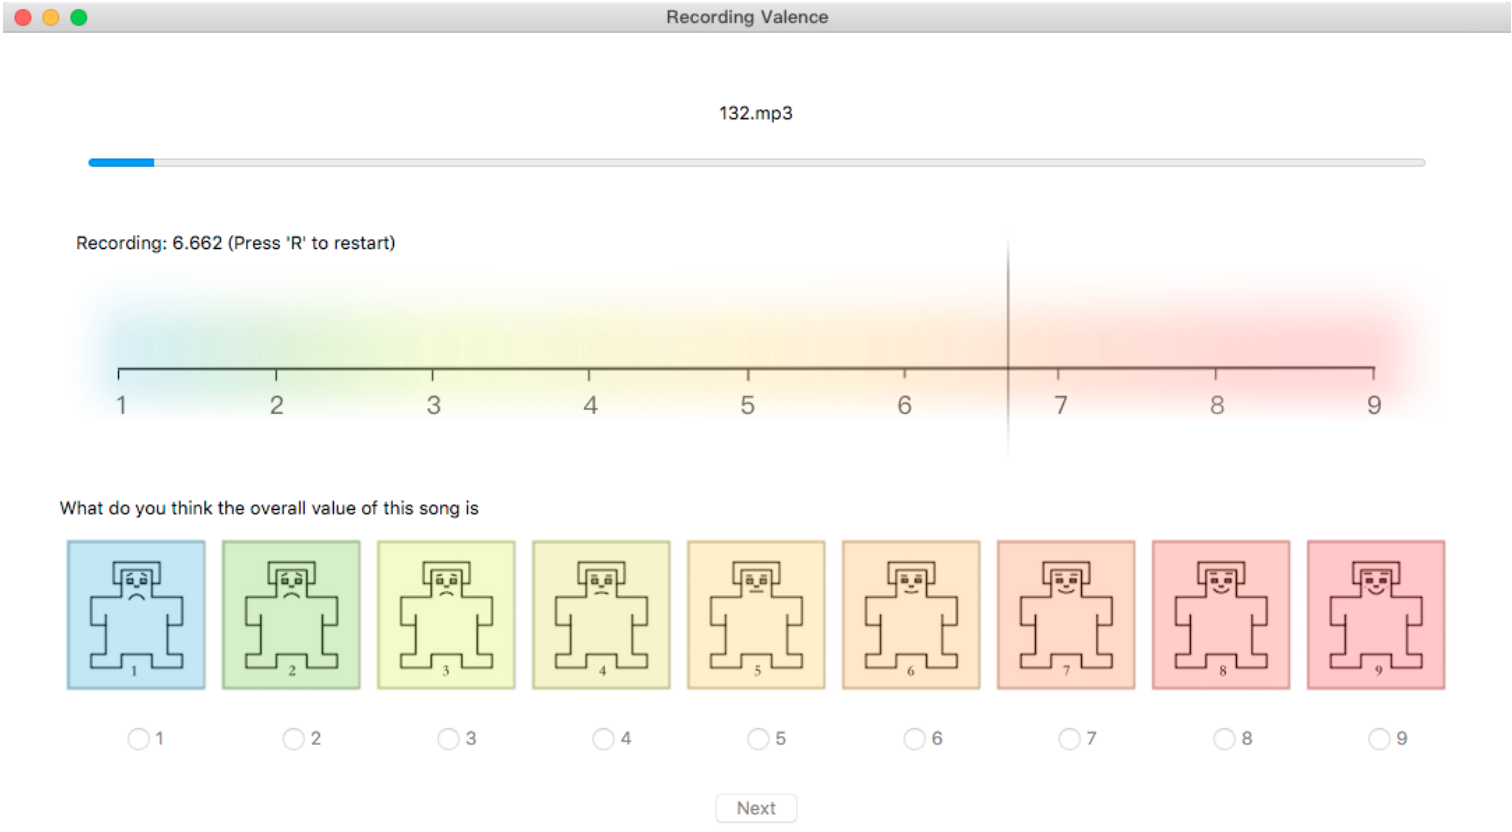
\includegraphics[width=0.65\textwidth]{annotation_interface.png} 
	\caption{Annotation interface for PMEmo}
    \label{fig:annotation_interface}
\end{figure}
\\
In figure \ref{fig:experimental_procedure} is shown the flow diagram of the experiment, where each subject spent $50$ minutes on average.
\begin{figure}[h]
    \centering
    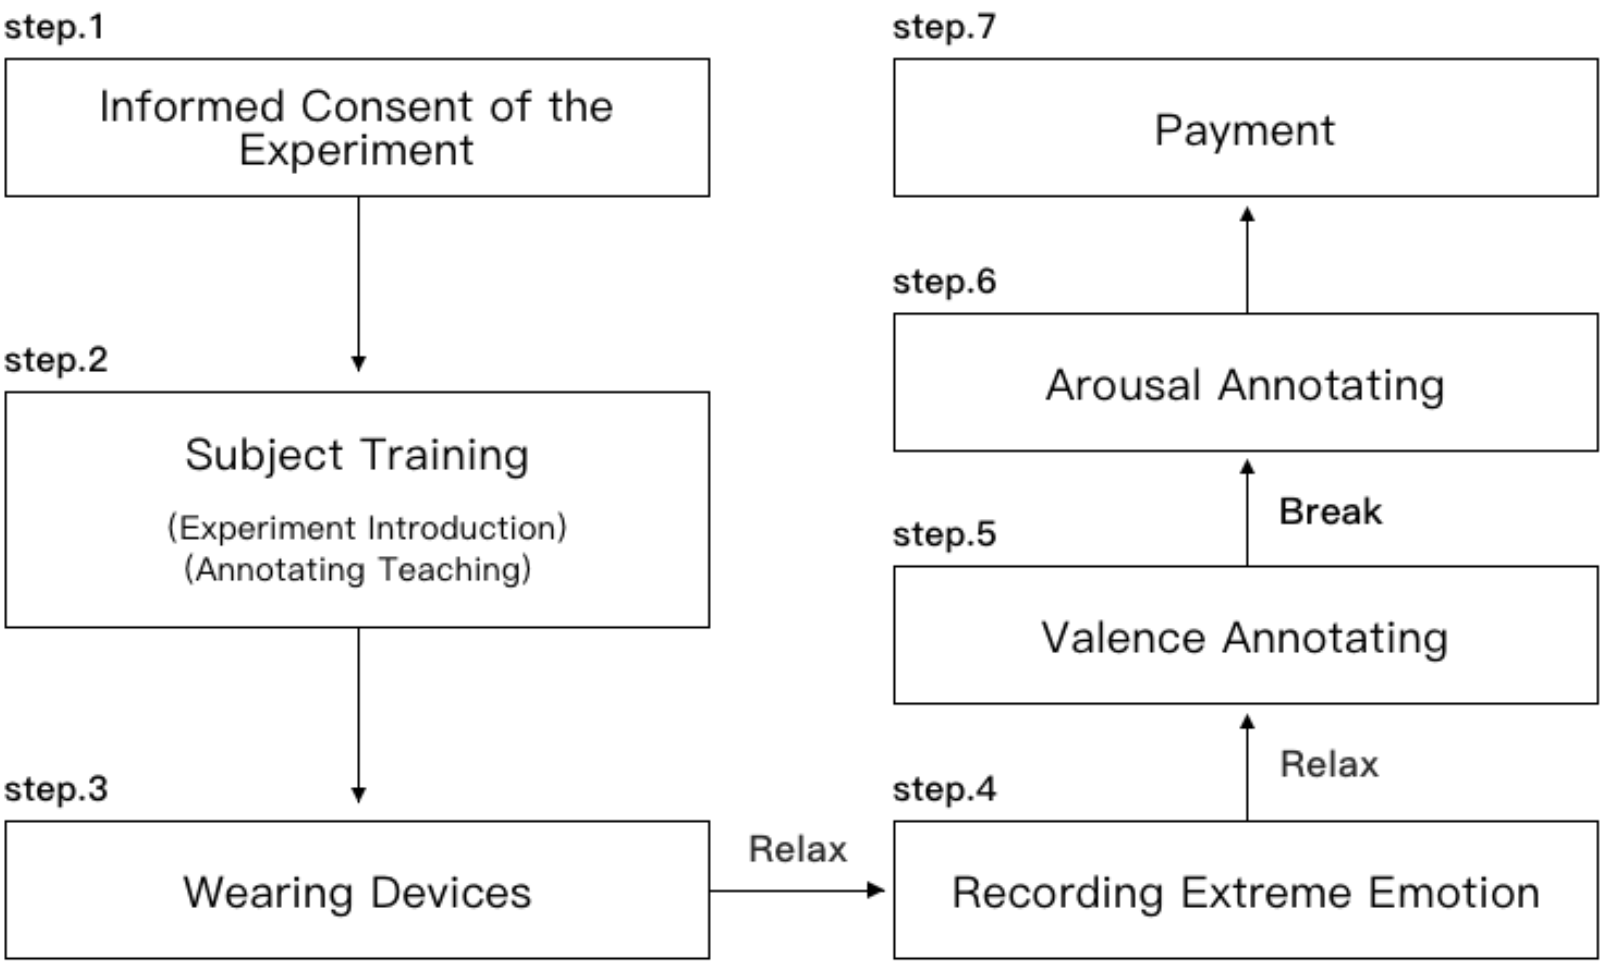
\includegraphics[width=0.7\textwidth]{experimental_procedure.png} 
	\caption{Experimental procedure for PMEmo}
    \label{fig:experimental_procedure}
\end{figure}
\\
Each subject listened to $20$ excerpts and one of those was duplicated to guarantee the high quality data as what was done in \cite{chen2015amg1608}. The annotations from this subjects were accepted only if the bias between duplicate clips were within $0.25$ in the \gls{va} space (they did not inform subjects about the duplicated excerpt).
\\
In total $457$ subjects have participated but $401$ were considered valid annotations ($87.7\%$). Each music clip was annotated by at least $10$ subjects including English speakers and semi-experts from music academy.

\subsection{Data reliability}
As \gls{iot} concept remarks, annotators need some preliminary time before they can give meaningful and reliable annotations. Schubert in \cite{schubert2013reliability} found that median \gls{iot} for valence was $8s$ while for arousal $12s$. Other researchers showed that annotations began to converge after $10s$. The \gls{pmemo} authors decided to discard first $15s$ for the dynamic annotations from the data.
\\ \indent
To evaluate annotation consistency they used the Chronbach's $\alpha$, it represent the degree to which a set of items measures a single unidimensional latent construct. In \cite{zhang2018pmemo} computed the Chronbach's $\alpha$ on the sequence of annotations for each song.
\\
They processed annotations by:
\begin{equation}
	a_{j,i}=a_{j,i}+(\bar{A}_j-\bar{A})
\end{equation}
where:
\begin{itemize}
	\item $a_{j,i}$ is the label annotated by subject $j$ at time $i$
	\item $\bar{A}$ is the mean of all the labels for this song by all subjects
	\item $\bar{A}_j$ is the mean of dynamic labels by subject $j$
\end{itemize}
The mean (averaged across songs) and the standard deviation of the Chronbach's $\alpha$ for the annotation in the \gls{pmemo} dataset are shown in table \ref{table:Chronbach}.
\begin{table}[h!]
	\centering
	\begin{tabular}{|c|c|c|}
		\hline
		Dimension & Mean & Std Dev \\ [0.5ex] 
		\hline\hline Valence & 0.998 & 0.005 \\ 
		\hline Arousal & 0.998 & 0.008 \\ 
		\hline
	\end{tabular}
	\caption{Mean and standard deviation of the Chronbach's $\alpha$ for PMEmo dataset annotations}
	\label{table:Chronbach}
\end{table}

\subsection{Feature set}
As already mentioned before in \ref{music_features}, for generic \gls{mer} there has been no attempt made at defining a "standard" feature set. In PMEmo work \cite{zhang2018pmemo} they based on the INTERSPEECH 2013 \gls{compare} \cite{schuller2013interspeech} and extracted a feature set of 6373-dimension scale.
\\
They provided all $6373$-dimension features in song level for the sake of static emotion task. They extracted only the core of $260$-dimension features in segment level (calculated in $1s$ window with $0.5s$ overlap) for dynamic recognition task to properly reduce the computing load.
\\
Extraction of the features is done with the open-source toolkit \href{https://www.audeering.com/opensmile/}{openSMILE}\footnote{https://www.audeering.com/opensmile/} \cite{eyben2013recent}.
\\
No feature selection procedure was implemented in \gls{pmemo} work.

\section{Implementation}
We decided to start from the results of \gls{pmemo} and try to improve them. We will first look at a general framework description and then will follow explanation of the single parts.

\subsection{General framework}
As already presented in chapter \ref{general_methodology} in figure \ref{fig:emotion_recognition_process} through some steps we can derive a model from the emotion elicitation. Since we will try to deal with both audio and \gls{eda} data, we decided to develop a model based on a traditional machine learning framework.
\\
General framework implemented is in figure \ref{fig:general_framework}. Differently from figure \ref{fig:emotion_recognition_process}, here, the starting point is dataset files given from the \gls{pmemo} dataset.
\begin{figure}[h]
    \centering
    \includegraphics[width=\textwidth]{general_framework.png} 
	\caption{General framework}
    \label{fig:general_framework}
\end{figure}
\\
From the dataset containing audio and \gls{eda} files, we extracted a certain number of features, creating a matrix for all the features extracted.
\\
From the feature matrix, several feature selection algorithms were applied in order to reduce the number of features, to improve the model.
\\
At last, some \gls{ml} process is applied to create the model for the emotion classification task and then it is tested.
\\
In this dataset were present two different types of data, audio and \gls{eda} and our main goal was to combine:
\begin{itemize}
	\item audio data,which gave the possibility to recognize perceived emotions
	\item \gls{eda} data, which are related to felt emotions
\end{itemize}
The general framework, with these two process divided is shown in figure \ref{fig:general_framework_1} which is based on the one presented before at \ref{fig:general_framework}.
\begin{figure}[h]
    \centering
    \includegraphics[width=\textwidth]{general_framework_1.png} 
	\caption{General framework with audio and EDA division}
    \label{fig:general_framework_1}
\end{figure}
\\[5px]
Now will be presented the first part of the general framework, feature extraction block, separated for audio and for \gls{eda}, due to evident differences in data types. For the audio, there are several set of features that can be extracted, thanks to the hard work done in the past years. While \gls{eda} features are less present in the literature and they are mostly statistical features.

\subsection{Audio feature extraction}
For the next features explanation, will be used the song contained in the \gls{pmemo} dataset under the name \textit{4.mp3}, \textit{X Bitch} from \textit{21 Savage} in the album "\textit{Savage mode}". Its waveform and audio specs can be seen in figure \ref{fig:audio_specs}.
\begin{figure}[h]
    \centering
    \includegraphics[width=\textwidth]{audio_specs.png} 
	\caption{Waveform and audio specs of the song number 4}
    \label{fig:audio_specs}
\end{figure}
\\
Now will follow a list of features extracted during the process.
\\
Features was extracted both in a static way, taking into account the whole excerpt and in a dynamic way, by dividing the musical excerpt in windows of $1s$ with $50\%$ overlap.
\\
After the process of feature extraction, every feature was normalized in the range $[0,1]$.
\paragraph{Tempo}
\mbox{} \\ \\
In musical terminology, tempo  is the speed or pace of a given piece. In classical music, tempo is typically indicated with an instruction at the start of a piece and is usually measured in beats per minute (or bpm).
\\
Tempo for the given song is about $152 bpm$.

\paragraph{Beats}
\mbox{} \\ \\
To extract beats is used a beat extractor, which output is an estimation of the tempo and an array of frame numbers corresponding to detected beat events.
\\
Beats are detected in three stages:
\begin{enumerate}	
	\item Measure onset strength
	\item Estimate tempo from onset correlation
	\item Pick peaks in onset strength approximately consistent with estimated tempo
\end{enumerate}
In figure \ref{fig:beat} can be seen beats detected and the array of frame numbers.
\begin{figure}[h]
    \centering
    \includegraphics[width=\textwidth]{beat.png} 
	\caption{Beat and array of frames of the song number 4}
    \label{fig:beat}
\end{figure}
\\
After the beats extraction, summation and average of the beat events are calculated.

\paragraph{Zero crossing rate}
\mbox{} \\ \\
The \gls{zcr}  is the rate of sign-changes along a signal. It is the rate at which the signal changes from positive to zero to negative or to negative or from negative to zero to positive. It is useful to recognize percussive sounds.
The \gls{zcr} is evaluated as:
\begin{equation}
	ZCR=\dfrac{1}{T} \sum_{t=1}^{T-1}{\dfrac{|sign(s_t)|-|sign(s_{t-1})|}{2}}
\end{equation}
where $T$ is the length of the time window, $s_t$ is the magnitude of the $t^{th}$ time domain sample.
\\
The \gls{zcr} of song 4 is shown in figure \ref{fig:zcr}.
\begin{figure}[h]
    \centering
    \includegraphics[width=\textwidth]{zcr.png} 
	\caption{ZCR extracted from song 4}
    \label{fig:zcr}
\end{figure}
\\
For the \gls{zcr}, is calculated the mean, the standard deviation, and the variance.

\paragraph{Chroma}
\mbox{} \\ \\
The chroma feature, also called chromagram, relates to the twelve different pitch classes. Chroma features capture harmonic and melodic characteristic of music, while being robust to changes in timbre and instrumentation.
\\
Humans perceive two musical pitches as similar if they differ by an octave. A pitch can be separated into two components, referred as \textit{height} (the octave where the pitch is) and \textit{chroma}. The twelve chroma values are represented by the set:
\[{C, C\#, D, D\#, E , F, F\#, G, G\#, A, A\#, B}\]
that consists of the twelve pitch spelling attributes as used in Western music notation.
\\
In the figure \ref{fig:chromagram} from \cite{inproceedings} can be seen a chromagram (b) obtained from the score (a) and a chromagram (d) obtained from an audio recording of the C-major scale played on a piano (c).
\begin{figure}[h]
    \centering
    \includegraphics[width=0.8\textwidth]{chromagram.png} 
	\caption{(a) Musical score of a C-major scale, (b) Chromagram obtained from the score, (c) audio recording of the C-major scale played on a piano, (d) chromagram obtained from the audio recording from \cite{inproceedings}}
    \label{fig:chromagram}
\end{figure}
\\
There are different ways to convert an audio recording into a chromagram, as performing \gls{stft} in combination with binning strategies or using multirate filter banks.
\\ \indent
Chroma features can be significantly changed by introducing pre-processing and post-processing steps that modify spectral, temporal and dynamical aspects. This leads to a large number of chroma variants.
\\
For the chromagram, we extracted three different types of chroma:
\begin{itemize}
	\item Chroma \gls{stft} extract the chromagram through the \gls{stft}.
	\item Chroma cqt extract the constant-Q chromagram, where the constant-Q transforms the data series to the frequency domain. Q stands for the quality factor, defined as:
	\begin{equation}
		Q=\dfrac{f_k}{\delta f_k}
	\end{equation}
	where $f_k$ is the $k^{th}$ filter while $\delta f_k$ is the bandwidth of the $k^{th}$ filter.
	\item Chroma cens which consider short-time statistics over energy distribution within the chroma bands. In \gls{cens} features, a quantization is applied based on logarithmic thresholds, which introduce a temporal smoothing.
\end{itemize}
In the figure \ref{fig:chroma} are shown the three different chromagram extracted for the song number 4.
\begin{figure}[h]
    \centering
    \begin{subfigure}{{\textwidth}}
    		\includegraphics[width=\textwidth]{chroma_stft.png}
    		\caption{Chroma stft}
    \end{subfigure}
    \begin{subfigure}{\textwidth}
    		\includegraphics[width=\textwidth]{chroma_cqt.png} 
    		\caption{Chroma cqt}
    \end{subfigure}
    \begin{subfigure}{\textwidth}
    		\includegraphics[width=\textwidth]{chroma_cens.png} 
    		\caption{Chroma cens}
    \end{subfigure}
    \caption{Different chromagram extracted from song number 4}
    \label{fig:chroma}
\end{figure}
\\
For every type of chromagram, is calculated the mean, the standard deviation, and the variance.

\paragraph{Melspectrogram}
\mbox{} \\ \\
The melspectrogram is a mel-scaled spectrogram. A spectrogram is a visual representation of the spectrum of frequencies of a signal as it varies with time. It can be generated by a bank of band-pass filter, by Fourier transform or \gls{dwt}.
\\ \indent
In order to have a more comprehensible spectrogram, when dealing with audio signals, it is scaled. The axis representing the frequencies is transformed to log scale, and the \textit{color} axis representing the amplitude, is scaled to Decibels, kinda of the log scale of amplitudes.
\\ \indent
The Mel-scale is a different scale, based on non-linear transformation of the frequency scale. It is constructed such that sounds of equal distance from each other on the Mel-scale also \textit{sound} to humans as they are equal in distance from one another.
\\
In practice it partitions the $Hz$ scale into bins, and transforms each bin into a corresponding bin in the Mel Scale, using a overlapping triangular filters.
\\
To convert a frequency in $Hz$ into its equivalent in $mel$, the following formula is used:
\begin{equation}
	pitch[mel]=1127.0148\:\log \left[ {1+\dfrac{f}{100}} \right]
\end{equation}
\\
Finally, a melspectrogram is a spectrogram with the mel-scale on the frequency axis.
\\
The melspectrogram of song 4 is shown in figure \ref{fig:melspectrogram}.
\begin{figure}[h]
    \centering
    \includegraphics[width=\textwidth]{melspectrogram.png} 
	\caption{Melspectrogram extracted from song 4}
    \label{fig:melspectrogram}
\end{figure}
\\
For the melspectrogram, is calculated the mean, the standard deviation, and the variance.

\paragraph{Spectral contrast}
\mbox{} \\ \\
Spectral contrast consider spectral peaks and valleys in each sub-band separately. More in general spectral peaks correspond to harmonic components and spectral valleys correspond to non-harmonic components or noise in a music piece as evaluated in \cite{jiang2002music}.
\\
Therefore, the difference between spectral peaks and spectral valleys will reflect the spectral contrast distribution.
\\
The spectral contrast of song 4 is shown in figure \ref{fig:spectral_contrast}.
\begin{figure}[h]
    \centering
    \includegraphics[width=\textwidth]{spectral_contrast.png} 
	\caption{Spectral contrast extracted from song 4}
    \label{fig:spectral_contrast}
\end{figure}
\\
For the spectral contrast, is calculated the mean, the standard deviation, and the variance.

\paragraph{Spectral centroid}
\mbox{} \\ \\
Spectral centroid is a measure to characterize a spectrum. It indicates where is located the center of mass of the spectrum. It has connection with the brightness of a sound.
\\
Spectral centroid is calculated as a weighted mean of the frequencies present in the signal, determined using a Fourier transform, with their magnitudes as the weights:
\begin{equation}
	cent=\dfrac{\sum_{n=0}^{N-1}{f(n)x(n)}}{\sum_{n=0}^{N-1}{x(n)}}
\end{equation}
where $x(n)$ is the weighted frequency value (or magnitude) of bin number $n$ and $f(n)$ represents the center frequency of that bin.
\\
The spectral centroid of song 4 is shown in figure \ref{fig:spectral_centroid}.
\begin{figure}[h]
    \centering
    \includegraphics[width=\textwidth]{spectral_centroid.png} 
	\caption{Spectral centroid extracted from song 4}
    \label{fig:spectral_centroid}
\end{figure}
\\
For the spectral centroid, is calculated the mean, the standard deviation, and the variance.

\paragraph{Spectral bandwidth}
\mbox{} \\ \\
The spectral bandwidth is the order-p spectral bandwidth as:
\begin{equation}
	{\left(\sum_{k}{S(k){(f(k)-f_c)}^p}\right)}^{1/p}
\end{equation}
where $S(k)$ is the spectral magnitude at frequency bin $k$, $f(k)$ is the frequency at bin $k$ and $f_c$ is the spectral centroid.
\\
The spectral bandwidth of song 4 is shown in figure \ref{fig:spectral_bandwidth}.
\begin{figure}[h]
    \centering
    \includegraphics[width=\textwidth]{spectral_bandwidth.png} 
	\caption{Spectral bandwidth extracted from song 4}
    \label{fig:spectral_bandwidth}
\end{figure}
\\
For the spectral bandwidth, is calculated the mean, the standard deviation, and the variance.

\paragraph{Spectral rolloff}
\mbox{} \\ \\
Spectral rolloff is defined as the $N^{th}$ percentile of the power spectral distribution, where $N$ is usually $85 \%$ or $95 \%$. The rolloff point is the frequency below which the N of the magnitude distribution is concentrated.
\\
This can be used to, e.g., approximate the maximum (or minimum) frequency by setting roll\_percent to a value close to $1$ (or $0$).
\\
The spectral rolloff of song 4 is shown in figure \ref{fig:spectral_rolloff}.
\begin{figure}[h]
    \centering
    \includegraphics[width=\textwidth]{spectral_rolloff.png} 
	\caption{Spectral rolloff extracted from song 4}
    \label{fig:spectral_rolloff}
\end{figure}
\\
For the spectral rolloff, is calculated the mean, the standard deviation, and the variance.

\paragraph{Spectral poly}
\mbox{} \\ \\
Get coefficients of fitting an $n^{th}$ order polynomial to the columns of a spectrogram.
\\
In the figure \ref{fig:poly} can be seen different poly extracted from song number 4, with different degrees, 0-order fit a degree-0 polynomial (constant) to each frame, 1-order fit a linear polynomial to each frame and 2-order fit a quadratic to each frame.
\begin{figure}[h]
    \centering
    \includegraphics[width=\textwidth]{poly.png} 
	\caption{Spectral poly extracted from song 4}
    \label{fig:poly}
\end{figure}
\\
For the spectral poly, is calculated the mean, the standard deviation, and the variance.

\paragraph{Tonal centroid}
\mbox{} \\ \\
Computes the tonal centroid features (tonnetz), following the method of \cite{harte2006detecting}.
\\
In musical tuning and harmony, the Tonnetz, is a conceptual lattice diagram representing tonal space first described by Euler in 1739. Various visual representations of the Tonnetz can be used to show traditional harmonic relationships in European classical music.
\\
Close harmonic relations are modeled as short distances on an infinite Euclidian plane. Chords become geometric structure on the plane and chords become geometric structures on the plane, keys are defined by regions in the harmonic network
\\
An example is shown in figure \ref{fig:tonnetz_scheme}.
\begin{figure}[h]
    \centering
    \includegraphics[width=\textwidth]{tonnetz_scheme.png} 
	\caption{Representation in the Euclidian plane of the tonnetz}
    \label{fig:tonnetz_scheme}
\end{figure}
\\
The Tonnetz of the song number 4 is shown in figure \ref{fig:tonnetz}.
\\
\begin{figure}[h]
    \centering
    \includegraphics[width=\textwidth]{tonnetz.png} 
	\caption{Tonnetz extracted in from song 4}
    \label{fig:tonnetz}
\end{figure}

\paragraph{Mel Frequency Cepstral Coefficients}
\mbox{} \\ \\
The \gls{mfcc} are coefficients based on the extraction of the signal energy within critical frequency bands by means of a series of triangular filters (in figure \ref{fig:mfcc_filters}) whose center frequencies are equally spaced according to the mel scale.
\begin{figure}[h]
    \centering
    \includegraphics[width=\textwidth]{mfcc_filters.png} 
	\caption{Triangular filters for the MFCC extraction}
    \label{fig:mfcc_filters}
\end{figure}
\\
The log-energy of the spectrum is measured within the pass-band of each filter, resulting in a reduced representation of the spectrum. The cepstral coefficients are finally obtained through a \gls{dct} of the reduced log-energy spectrum.
\\
In figure \ref{fig:mfcc} is shown the \gls{mfcc} graph for 12 mfccs for song number 4.
\begin{figure}[h]
    \centering
    \includegraphics[width=\textwidth]{mfcc.png} 
	\caption{MFCC for song 4}
    \label{fig:mfcc}
\end{figure}
\\
For each of the $12$ \gls{mfcc}s are extracted the mean, standard deviation, median, kurtosis and skewness.

\subsection{EDA feature extraction}
For the continuity, also in the explanation of \gls{eda} features extracted, will be used the song number 4. Its \gls{eda} signal and its specs, can be seen in figure \ref{fig:eda}.
\begin{figure}[h]
    \centering
    \includegraphics[width=\textwidth]{eda.png} 
	\caption{EDA for song 4}
    \label{fig:eda}
\end{figure}
\\
\gls{eda} signal was preprocessed following the pipeline highlighted in the pyphysio library \cite{bizzego2019pyphysio} and resumed in figure \ref{fig:pyphysio_pipeline}.
\begin{figure}[h]
    \centering
    \includegraphics[width=\textwidth]{pyphysio_pipeline.png} 
	\caption{Pyphysio pipeline}
    \label{fig:pyphysio_pipeline}
\end{figure}
\\
They divide the pipelines into three separate steps:
\begin{enumerate}
	\item Filtering and Preprocessing: this step includes all the procedures aiming at increasing the signal/noise ratio, typycally band-pass filtering, smoothing, removal of artifacts. The output of this step is a new version of the imput signal with improved signal quality (less noise)
	\item Information Extraction: this step aims at extracting the information of interest from the physiological signal. The output is a new signal containing only the information of interest and thus it has a signal\_nature different from the input signal
	\item Physiological Indicators: this steps produces a list of scalar values able to describe the characteristics of the input signal. This step is usually performed on small segments of the input signals which are extracted using a sliding window on the whole length of the signal.
\end{enumerate}
Taking into account the initial signal shown in figure \ref{fig:eda} the filtering and preprocessing stage was done by an \gls{iir} filter to remove high frequency noise, a low-pass filter of $0.6Hz$ to diminuish the noise from motion and artifacts as can be seen in figure \ref{fig:eda_filtered}.
\begin{figure}[h]
    \centering
    \includegraphics[width=\textwidth]{eda_filtered.png} 
	\caption{EDA signal in blue and filtered EDA in orange}
    \label{fig:eda_filtered}
\end{figure}
\\
Following the procedure introduced by \cite{bizzego2019pyphysio}, the library is able to extract tonic and phasic component of an \gls{eda} data by evaluating a driver function. The graph can be seen in figure \ref{fig:eda_phasic_driver}.
\begin{figure}[h]
    \centering
    \includegraphics[width=\textwidth]{eda_phasic_driver.png} 
	\caption{EDA signal in blue, driver in orange and tonic part in green}
    \label{fig:eda_phasic_driver}
\end{figure}
\\
Now will follow a list of features extracted during the process.
\\
Features was extracted both in a static way, taking into account the whole excerpt and in a dynamic way, by dividing the musical excerpt in windows of $1s$ with $50\%$ overlap.
\\
After the process of feature extraction, every feature was normalized in the range $[0,1]$.

\paragraph{Statistic}
\mbox{} \\ \\
As already mentioned before in \ref{EDA_features}, most extracted \gls{eda} features are statistical. We extracted the mean of the signal, the standard deviation, kurtosis and the skewness. They were extracted both in the time domain and in the frequency domain.
\\ \indent
Median value was also extracted, where the median is the value separating the higher half from the lower half of the data. It is like the \textit{middle} value, but differently from the mean, the median gives a better idea of a typical value.
\\
While other statistics were already described in \ref{EDA_features}, the median can be described in a caseless formula as:
\begin{equation}
	median(a)=\dfrac{a_{\left \lceil{\dfrac{l+1}{2}}\right \rceil}+a_{\left \lfloor{\dfrac{l+1}{2}}\right \rfloor}}{2}
\end{equation}
where $a$ is an ordered list of $l$ numbers, $\left \lceil {\cdot} \right \rceil$ is the ceil function (gives the least integer greater than or equal to the input) and $\left \lfloor {\cdot} \right \rfloor$ is the floor function (gives the greatest integer less than or equal to the input).
\\ \indent
We extracted also the maximum value, the minimum and the difference between these two, the range.

\paragraph{Other features}
\mbox{} \\ \\
Some other features were extracted thanks to pyphisio library \cite{bizzego2019pyphysio}, they are:
\begin{itemize}
	\item \gls{auc}
	\item \gls{rmssd} compute the \gls{rmse} of the squared $1^{st}$ order discrete differences
	\item \gls{sdsd} calculate the standard deviation of the $1^{st}$ order discrete differences
\end{itemize}

\paragraph{Power and Peak inband}
\mbox{} \\ \\
The power spectrum $S_{xx}(f)$ of a time series $x(t)$ describes the distribution of power into frequency components compsing the signal. Any discrete signal, according to Fourier analysis, can be decomposed into a number of discrete frequencies, or a spectrum of frequencies over a continuous range.
\\
The statistical average of a certain signal as analyzed in terms of its frequency content, is called its spectrum.
\\ \indent
The \gls{psd}, also called power spectrum, applies to signal over all time, that theoretically could be an infinite time interval. The \gls{psd} than, refers to the spectral energy distribution that would be found per unit time, since the total energy of such a signal over all time would generally be infinite.
\\
We extracted the power and the peak frequency for each frequency band. We decided to set the same frequency ranges as in \gls{pmemo}:
\begin{itemize}
	\item $0Hz-0.1Hz$
	\item $0.1Hz-0.2Hz$
	\item $0.2Hz-0.3Hz$
	\item $0.3Hz-0.4Hz$
	\item $0.4Hz-0.5Hz$
\end{itemize}

\paragraph{Mel Frequency Cepstral Coefficients}
\mbox{} \\ \\
As for the audio features, we extracted \gls{mfcc} features. We kept $12$ \gls{mfcc} coefficients.
\\
For each of the $12$ \gls{mfcc}s are extracted the mean, standard deviation, median, kurtosis and skewness.

\subsection{Feature selection}\label{feature_selection_5}
Feature selection become an important step while performing a \gls{ml} task. Given a dataset, every column of the dataset is a feature, and not necessarily every feature is going to have an impact on the output variable.
\\
Adding these irrelevant features in the model, it will make the model worst.
\\
These feature selection methods are valid for a regression problem, where both the input and the output variables are continuous in nature.
\\ \indent
Feature selection can be done in multiple ways but there are broadly 3 categories of it:
\begin{enumerate}
	\item Filter Method by filtering and taking only the subset of the relevant features, the filtering is done using correlation matrices. 
	\item Wrapper Method which needs a \gls{ml} algorithm and uses its performance as evaluation criteria.
	\item Embedded Method in an iterative way, it takes care of each iteration of the model training process and extract those features which contribute the most to the training for a particular iteration.
\end{enumerate}
In the following paragraphs are taken into account all the audio features extracted for the whole song, in the static case.

\paragraph{Pearson correlation}
\mbox{} \\ \\
Pearson correlation is a filter method for feature selection. In this method a filter process is done which select only the subset of the relevant features. The model is built after selecting the features.
\\
The filtering is done using Pearson correlation.
\\ \indent
In statistics, the Pearson correlation coefficient is a measure of the linear correlation between two variables $X$ and $Y$.
\\
The correlation coefficient has values between -1 to 1:
\begin{itemize}
	\item A value closer to $0$ implies weaker correlation (exact $0$ implying no correlation)
	\item A value closer to $1$ implies stronger positive correlation
	\item A value closer to $-1$ implies stronger negative correlation
\end{itemize}
Pearson's correlation coefficient is the covariance of the two variables divided by the product of their standard deviations. The form of the definition involves a \textit{product moment}, that is, the mean (the first moment about the origin) of the product of the mean-adjusted random variables:
\begin{equation}
	\rho_{X,Y}=\dfrac{cov(X,Y)}{\sigma_X \sigma_Y}
\end{equation}
where:
\begin{itemize}
	\item $cov(X,Y)$ is the covariance (the measure of the joint variability of the two random variables $X$ and $Y$)
	\item $\sigma_X$ is the standard deviation of $X$
	\item $\sigma_Y$ is the standard deviation of $Y$
\end{itemize}
In figure \ref{fig:Pearson_heatmap} is shown the Pearson correlation heatmap, which represents the correlation of independent variables with the output variable.
\begin{figure}[h]
    \centering
    \includegraphics[width=\textwidth]{Pearson_heatmap.png} 
	\caption{Pearson heatmap}
    \label{fig:Pearson_heatmap}
\end{figure}
\\
Then are selected just the features that have a Pearson coefficient greater than a certain value, for example features that have a Pearson coefficient greater than $0.5$ based on the output variable of \textit{Valence (mean)} are shown in figure \ref{fig:Pearson_features}.
\begin{figure}[h]
    \centering
    \includegraphics[width=0.8\textwidth]{Pearson_features.png} 
	\caption{Pearson most relevant features}
    \label{fig:Pearson_features}
\end{figure}

\paragraph{Backward elimination}
\mbox{} \\ \\
Backward elimination is a wrapper feature selection method. The model is fed at first with all the features, than is check the performance of the model and iteratively is removed the worst performing features one by one till the overall performance of the model comes in acceptable range.
\\
The performance metric used here to evaluate feature performance is pvalue. If the pvalue is above $0.05$ then we remove the feature, else it is kept.
\\
Features that have a pvalue smaller than $0.05$ are:
\\ \linebreak 
\textit{['chroma\_cq\_mean', 'chroma\_cq\_std', 'chroma\_cq\_var', 'chroma\_cens\_mean', 'melspectrogram\_mean', 'cent\_mean', 'contrast\_mean', 'contrast\_std', 'tonnetz\_std', 'tonnetz\_var', 'harm\_var', 'perc\_std', 'frame\_std', 'frame\_var', 'meanMFCC[0]', 'stdMFCC[0]', 'skewMFCC[0]', 'medianMFCC[1]', 'skewMFCC[1]', 'meanMFCC[2]', 'medianMFCC[2]', 'stdMFCC[3]', 'medianMFCC[3]', 'skewMFCC[3]', 'kurtMFCC[4]', 'skewMFCC[4]', 'stdMFCC[5]', 'medianMFCC[5]', 'skewMFCC[5]', 'meanMFCC[7]', 'stdMFCC[8]', 'medianMFCC[8]', 'meanMFCC[9]', 'meanMFCC[11]', 'mfcc\_delta\_std', 'mfcc\_delta\_var']}

\paragraph{Recursive feature elimination}
\mbox{} \\ \\
The \gls{rfe} method is another wrapper method and works by recursively removing attributes and building a model on those attributes that remain.
\\
It uses accuracy metric to rank the feature according to their importance. The \gls{rfe} method takes the model to be used and the number of required features as input. As output it gives the ranking of all the variables, where $1$ is the most important.
\\
Most relevant features extracted are:
\\ \linebreak 
\textit{['chroma\_stft\_mean', 'chroma\_stft\_std', 'chroma\_stft\_var', 'chroma\_cq\_mean', 'chroma\_cq\_std', 'chroma\_cq\_var', 'chroma\_cens\_mean', 'chroma\_cens\_std', 'chroma\_cens\_var', 'melspectrogram\_mean', 'contrast\_mean', 'contrast\_std', 'contrast\_var', 'poly\_mean', 'poly\_std', 'poly\_var', 'tonnetz\_mean', 'tonnetz\_std', 'tonnetz\_var', 'zcr\_mean', 'zcr\_std', 'zcr\_var', 'harm\_mean', 'harm\_std', 'harm\_var', 'perc\_mean', 'perc\_std', 'perc\_var', 'frame\_mean', 'frame\_std',  'frame\_var', 'meanMFCC[0]', 'stdMFCC[0]', 'kurtMFCC[0]', 'skewMFCC[0]', 'meanMFCC[1]', 'medianMFCC[1]', 'kurtMFCC[1]', 'skewMFCC[1]', 'meanMFCC[2]', 'stdMFCC[2]', 'medianMFCC[2]', 'kurtMFCC[2]', 'skewMFCC[2]', 'meanMFCC[3]', 'stdMFCC[3]', 'medianMFCC[3]', 'kurtMFCC[3]', 'skewMFCC[3]', 'meanMFCC[4]', 'stdMFCC[4]', 'medianMFCC[4]', 'kurtMFCC[4]', 'skewMFCC[4]', 'meanMFCC[5]', 'stdMFCC[5]', 'medianMFCC[5]', 'kurtMFCC[5]', 'skewMFCC[5]', 'meanMFCC[6]', 'medianMFCC[6]', 'kurtMFCC[6]', 'skewMFCC[6]', 'meanMFCC[7]', 'stdMFCC[7]', 'medianMFCC[7]', 'kurtMFCC[7]', 'skewMFCC[7]', 'meanMFCC[8]', 'stdMFCC[8]', 'medianMFCC[8]',  'kurtMFCC[8]', 'skewMFCC[8]', 'meanMFCC[9]', 'stdMFCC[9]', 'medianMFCC[9]', 'kurtMFCC[9]', 'skewMFCC[9]', 'meanMFCC[10]', 'stdMFCC[10]', 'medianMFCC[10]', 'kurtMFCC[10]', 'skewMFCC[10]', 'meanMFCC[11]', 'stdMFCC[11]', 'medianMFCC[11]', 'kurtMFCC[11]', 'skewMFCC[11]', 'mfcc\_delta\_mean', 'mfcc\_delta\_std', 'mfcc\_delta\_var']}

\paragraph{Embedded method}
\mbox{} \\ \\
Embedded methods are iterative in a sense that takes care of each iteration of the model training process and carefully extract those features which contribute the most to the training for a particular iteration. Regularization methods are the most commonly used embedded methods which penalize a feature given a coefficient threshold.
Here we will do feature selection using Lasso regularization. If the feature is irrelevant, lasso penalizes its coefficient and make it $0$. Hence the features with coefficient equal to $0$ are removed and the rest are taken.
\\
Most relevant features extracted are:
\\ \linebreak 
\textit{['rolloff\_var', 'cent\_var', 'total\_beats', 'melspectrogram\_var', 'spec\_bw\_var'}

\paragraph{RReliefF}
\mbox{} \\ \\
As already explained in \ref{feature_selection}, the RReliefF algorithm is based on the quality estimation of each features, between instances that are close each other.
\\
The main benefit of Relief-based algorithms is that they identify feature interactions without having to exhaustively check every pairwise interaction, thus taking significantly less time than exhaustive pairwise search.
\\
In this case, features were automatically ordered given a score, based on the RReliefF algorithm and a random forest classifier with $100$ estimators. In this implementation, as input of the function we need to specify the number of features we want to keep.
\\
Features selected with this method are:
\\ \linebreak 
\textit{['stdMFCC[0]',	 'rolloff\_var', 'chroma\_cens\_mean', 'chroma\_cens\_std', 'meanMFCC[1]', 'frame\_var', 'chroma\_cq\_var', 'poly\_mean', 'poly\_std', 'melspectrogram\_var']}

\subsection{Machine Learning methods}
The task of \gls{mer} is a problem that can be classified in the field of supervised \gls{ml}, because we have an input variable $x$, the song, and an output variable $Y$, the emotion, and we want to find an algorithm that lean the mapping function from the input to the output, $Y=f(x)$.
\\ \indent
General goal is to approximate the mapping function so well that when there is a new input, the algorithm can predict the output data.
\\
Supervised \gls{ml} is divided in two categories, regression and classification. The main difference between the two tasks is the fact that the dependent attribute is numerical for regression and categorical for classification.
\\ \indent
A regression problem is when the output variable is a real or continuous value. Many different models can be used. They are explained in detail in the following paragraphs.

\paragraph{Linear Regression}
\mbox{} \\ \\
\gls{lr} is a type of regression analysis where the number of independent variables is one and there is a linear relationship between the independent $x$ and the dependent one $y$.
\\
The figure \ref{fig:linear_regression} show a red line referred to the best fit straight line. Dots are the data points and the task of \gls{lr} is to try to plot a line that models the points the best.
\begin{figure}[h]
    \centering
    \includegraphics[width=0.8\textwidth]{linear_regression.png} 
	\caption{Linear regression}
    \label{fig:linear_regression}
\end{figure} 
\\
The line can be modeled based on the linear equation:
\begin{equation}
	y=a_0+a_1\cdot x
\end{equation}
Aim of \gls{lr} is to find the best value for $a_0$ and $a_1$. This is a search problem, which can be converted into a minimization problem where we would like to minimize the error between the predicted value and the actual one.
\\
The minimization problem is the cost function $J$:
\begin{equation}
	minimize \: \dfrac{1}{n} \sum_{i=1}^n{{(pred_i-y_i)}^2}
\end{equation}
\begin{equation}
	J=\dfrac{1}{n} \sum_{i=1}^n{{(pred_i-y_i)}^2}=\dfrac{1}{n} \sum_{i=1}^n{{(a_0+a_1\cdot x_i-y_i)}^2}
\end{equation}
To update $a_0$ and $a_1$ values in order to reduce the cost function $J$ is used the gradient descent, which idea is to start with random values of $a_0$ and $a_1$ and then iteratively update the values reaching minimum cost.

\paragraph{Lasso}
\mbox{} \\ \\
\gls{lasso} is a regression analysis method that performs both variable selection and regularization in order to enhance the prediction accuracy and interpretability of the statistical model it produces.
Taking into account a linear model based on $n$ features represented as:
\begin{equation}
	\hat{y}=w[0]x[0]+w[1]x[1]+...+w[n]x[n]+b
\end{equation}\label{linear_model}
Assuming the dataset has $M$ instances and $p$ values, the cost function of the regression problem can be written as:
\begin{equation}
	J=\sum_{i=1}^{M}{{(y_i-\hat{y}_i)}^2}=\sum_{i=1}^{M}{{ \left( y_i-\sum_{j=0}^{p}{w_jx_{ij}} \right) }^2}
\end{equation}\label{regression_eq}
The \gls{lasso} cost function can be written as:
\begin{equation}
	J=\sum_{i=1}^{M}{{(y_i-\hat{y}_i)}^2}=\sum_{i=1}^{M}{{ \left( y_i-\sum_{j=0}^{p}{w_jx_{ij}} \right) }^2}+\lambda \sum_{j=0}^{p}{|w_j|}
\end{equation}\label{lasso_eq}
It is evident that for $\lambda=0$, the equation \ref{eq:lasso_eq} reduces to equation \ref{eqregression_eq}. Here are taken in account the magnitude of the coefficients $w_j$.
\\
\gls{lasso} can have zero coefficient, which lead to neglecting some features for the evaluation of the output. This help as a feature selection step. Feature selection using \gls{lasso} regression can be depicted well by changing the regularization parameter $\lambda$. This is called $L_2$ regularization.

\paragraph{Ridge}
\mbox{} \\ \\
Ridge is another regression analysis method, similar to \gls{lasso}. Assuming the linear model described before in \ref{eq:linear_model}, the cost function for Ridge is:
\begin{equation}
	J=\sum_{i=1}^{M}{{(y_i-\hat{y}_i)}^2}=\sum_{i=1}^{M}{{ \left( y_i-\sum_{j=0}^{p}{w_jx_{ij}} \right) }^2}+\lambda \sum_{j=0}^{p}{{(w_j)}^2}
\end{equation}\label{ridge_eq}
Where is added a penalty equivalent to square of the magnitude of the coefficients $w_j$. This is called $L_1$ regularization.
\\
The penalty term $\lambda$ regularizes the coefficients such that if the coefficients take large value the optimization function is penalized. So, it shrinks the coefficients and helps to reduce model complexity.

\paragraph{Elastic Net}
\mbox{} \\ \\
Elastic Net is a regularized regression that linearly combines the $L_1$ and $L_2$ penalties of the Ridge and \gls{lasso} methods. Absolute value penalization and squared penalization are combined with a coefficient, $L_{r}$
\begin{equation}
	J=\sum_{i=1}^{M}{{ \left( y_i-\sum_{j=0}^{p}{w_jx_{ij}} \right) }^2}+(1-r) \lambda \sum_{j=0}^{p}{{(w_j)}^2}+r \lambda \sum_{j=0}^{p}{{(w_j)}^2}
\end{equation}\label{elasticnet_eq}

\paragraph{k-nearest neighbors}
\mbox{} \\ \\
The \gls{knn} algorithm, is a non-parametric algorithm used for regression, where input consists of the $k$ closest training examples in the feature space and the output is the property value for the object. This value is the average of the values of $k$ nearest neighbors.
\\
\gls{knn} is sensitive to the local structure of the data.

\paragraph{Support Vector}
\mbox{} \\ \\
Goal of a regression problem is to minimize the error rate. In \gls{svr} tries to fit the error within a certain threshold.
\\
The error term is handled in constraints by setting the absolute error less than or equal to a specified margin, called maximum error $\varepsilon$. The problem is a minimization proble $minimize \: \dfrac{1}{2}||w||^2$ with the constraint $|y_i-w_ix_i| \leq \varepsilon$ showed in figure \ref{fig:support_vector_regression}.
\begin{figure}[h]
    \centering
    \includegraphics[width=0.8\textwidth]{support_vector_regression.png} 
	\caption{Support Vector regression}
    \label{fig:support_vector_regression}
\end{figure} 

\paragraph{Decision Tree}
\mbox{} \\ \\
\gls{dt} is a supervised \gls{ml} problem used to predict a target by learning decision rules from features. Its model is based on a data division by making a decision based on asking a series of questions.
\\ \indent
\gls{dt} is constructed by recursive partitioning, starting from the root node, and then each node can be split into left and right child nodes. These nodes can then be further split and they themselves become parent nodes of their resulting children nodes.

\paragraph{Random Forest}
\mbox{} \\ \\
Random forest is a Supervised Learning algorithm which uses ensemble learning method for classification and regression.
\\
An ensemble method combines the predictions from multiple \gls{ml} algorithms together to make more accurate predictions.
\\
Figure \ref{fig:random_forest} show an ideal representation of \gls{rf}.
\begin{figure}[h]
    \centering
    \includegraphics[width=\textwidth]{random_forest.png} 
	\caption{Random Forest regression}
    \label{fig:random_forest}
\end{figure} 
\\
\gls{rf} operates by constructing a multitude of decision trees at training time and outputting the class that is the mean prediction of the individual trees.
\\
\gls{rf} allows to aggregate many \gls{dt} and this gives the possibility to split the features but limited to some percentage of the total (the hyperparameter). This allows to have a balanced weight on all the features.

\subsection{Evaluation parameters}
To evaluate how much the \gls{ml} model is precise and correct we used two different parameters, the \gls{rmse} and the coefficient of determination $R^2$.
\\ \indent
For both cases, to evaluate the score we applied a cross-validation with $10$ fold to train the data and one remaining to test the data.
\\
A division example is shown in figure \ref{fig:cross_validation}.
\begin{figure}[h]
    \centering
    \includegraphics[width=0.6\textwidth]{cross_validation.png} 
	\caption{k-fold cross validation}
    \label{fig:cross_validation}
\end{figure} 
\\
A well-fitting regression model results in predicted values close to the observed data values.
\\
The \gls{rmse} is the square root of the variance of the residuals. It indicates the absolute fit of the model to the data, how much close the observed data points are to the model's predicted values. \gls{rmse} is an absolute measure of fit. It is a good measure of how accurately the model predicts the response, and it is the most important criterion for fit if the main purpose of the model is prediction.
\\ \indent
$R^2$ is a statistical measure that represents the proportion of the variance for a dependent variable that is explained by variables in a regression model.
\\
It scales from $0$ to $1$ where $0$ indicates that the proposed model does not improve prediction over the mean model and $1$ indicates the perfect prediction. It can be also negative, in the case where the model can be arbitrarily worse.